\chapter{Introduction}\label{chap:introduction}

\section{The Challenge of Environmental Pollution}

Over the past few decades, the upsurge in environmental pollution by chemical compounds has been driven by industrial processes, agricultural methods, consumerism and various other contributing factors. Although these chemicals are integral for many products and have the potential to improve the comfort of modern society, they can also pose risks and adversely affect both human health and the environment, either acutely or chronically. Toxic substances threaten wildlife but also make air, soil, drinking water and food supply less safe. 

Nations worldwide maintain comprehensive chemical regulations\footnote{For instance, REACH, short for Registration, Evaluation, Authorisation, and Restriction of Chemicals, is an EU regulation aimed at improving chemical safety and allocating risk management responsibilities to companies operating in various sectors.}, however, it is anticipated that global chemicals production will double by 2030~\cite{chemicaloutlook}. Moreover, the widespread utilization of chemicals, including their inclusion in consumer goods, is expected to expand further.
Even though there are over 275 million known chemical compounds registered by the \emph{Chemical Abstracts Service}~\cite{CAS}, merely a tiny fraction of them undergo close monitoring via target analytical approaches and even less is known about their toxicity profiles and negative health effects on organsims. Table~\ref{tab:ubiquitous_water_pollutants} provides an overview of omnipresent water pollutants.

\begin{table}[h]
    \begin{tabularx}{\linewidth}{XXXX}
    \toprule
    Origin/Usage & Class & Examples & Related Issues \\
    \toprule
    Industrial\newline Chemicals & Solvents & Tetrachloro-methane & Drinking-water-quality \\
    & Intermediates & Methyl-t-butylether & Drinking-water-
    quality \\ 
    & Petrochemicals & BTEX (benzene, toluene, xylene) & Cancer \\ \midrule
    Industrial\newline Products & Additives & Phthalates & Endocrine disruptors \\
     & Lubricants & PCBs & Biomagnification \\
     & Flame Retardants & PBDEs & \\ \midrule
    Consumer\newline Products & Detergents & Nonylphenol ethoxylates & Endocrine effects \\
     & Pharmaceuticals & Antibiotics & Bacterial resistance \\
     & Hormones & Ethinyl estradiol & Feminization of fish \\ \midrule
     Biocides & Pesticides & DDT & Toxic effects and persistent metabolites \\
     & Nonagricultural biocides & Tributyltin & Endocrine effects \\ \midrule
    Geogenic \& \newline Natural\newline Chemicals & Heavy Metals & Lead, cadmium, mercury & Organ damage \\
     & Inorganics & Arsenic, selenium, fluoride & Drinking-water-quality\\
     & Taste and Odor & Geosmin & \\
     & Human Hormones & Estradiol & Feminization of fish \\ \midrule
    Disinfection \& \newline Oxidation & Disinfection by-products & Haloacetic acids, Bromate & Drinking-water-quality \\ \midrule
     Transformation Products & Metabolites from all above & Metabolites of perfluorinated compounds & Bioaccumulation\\
     & & Chloroacetanilide herbicide metabolites & Drinking-water-quality \\
    \bottomrule
    \end{tabularx}
    \caption{Table 2 adapted from~\cite{schwarzenbach2006}. Examples of ubiquitous water pollutants.}~\label{tab:ubiquitous_water_pollutants}
\end{table}


In light of the rapidly evolving chemical landscape, there is an increasing demand for future-proof, robust measurement and modeling methods. These methods are essential for evaluating the toxicity and exposure of chemicals, facilitating  informed risk-based decision-making even when data on hazards and exposures are limited. It is worth noting that the need for adaptable approaches in chemical safety and sustainability efforts must also prioritize cost-efficiency and gain widespread acceptance among regulatory bodies, industry stakeholders, and the general public.

For instance, the EU has introduced the 8th Environment Action Programme, as outlined in its European Green Deal~(cite{greendeal}), to provide direction for European environmental policy until the year 2030. This program reinforces the EU's ambitious goal of sustainable living within planetary limits, with a forward-looking vision that extends to 2050. Central to this vision is a zero-pollution commitment, encompassing air, water, and soil quality, all while prioritizing the well-being of EU citizens. In 2021, the European Commission introduced a sustainability-focused chemicals strategy~\cite{EUChemicalsStrategy}, which aligns with the EU's zero-pollution ambition. This strategy not only enables the evaluation of the safety and sustainability of both existing and future chemical compounds but also aims to reduce concerning substances, such as \emph{per- and polyfluoroalkyl substances (PFAS)}, through substitution or phasing out wherever feasible. In parallel, the \emph{U.S. Environmental Protection Agency (EPA)} shares a similar scientific consensus and is at the forefront of assessing the potential impacts of chemicals on human health and the environment. Leveraging advanced toxicological and exposure methods, EPA actively promotes risk reduction efforts through its own \emph{Chemical Safety for Sustainability National Research Program}. This program builds upon the achievements of research initiatives like \emph{ToxCast}\footnote{\url{https://www.epa.gov/comptox/toxcast}}, \emph{Tox21}\footnote{\url{https://tox21.gov/}}, and the Endocrine Disruptor Screening Program in the 21st Century (EDSP21), demonstrating a commitment to advancing chemical safety on a global scale.


\section{The Imperative for Prioritization and Toxicity Assessment}

Contemporary analytical techniques, including \emph{high-resolution mass spectrometry (HRMS/MS)}, are gaining significance across various domains such as metabolomics, drug discovery, environmental science and toxicology~\cite{tamara2022}. The application of nontarget HRMS/MS has notably improved the ability to detect unidentified emerging contaminants from environmental samples, often with unknown toxicity profiles. In the past, when it comes to prioritizing unidentified compounds, the standard approach has been to use signal intensity from the fragmentation data of tandem mass spectrometery (referred to as MS/MS or MS2). We now abbreviate this as MS2 for convenience. However, this approach tends to fall short in delivering an accurate assessment of environmental exposures because MS2 signal intensity may not relate proportionally to the compound's concentration in the sample. Furthermore, and of central importance to this work, this approach overlooks the toxicological factors essential for prioritizing compounds with concers related to environmental hazards. As a result, substances with the potential for severe ecological consequences, such as endocrine-disrupting compounds, often go undetected because of their low abundance, even though they exhibit high levels of toxicity. Hence, a pressing need exists for alternative approaches to prioritize unidentified nontarget HRMS/MS signals based on their hazard potential. Incorporating relevant toxicity considerations into the equation:

\begin{equation}
    \text{Risk} = \text{Hazard} \times \text{Exposure}
\end{equation}

augments our capacity to make well-informed decisions when evaluating the environmental risk associated with chemicals.
Figure~\ref{fig:non_target_high_resolution_mass_spectrometry} illustrates the non-target screening with \emph{HRMS/MS} technique and the novel prioritization \emph{} approach.
 
\begin{figure}[htbp]  % Placement options: h (here), t (top), b (bottom), p (page)
    \centering
    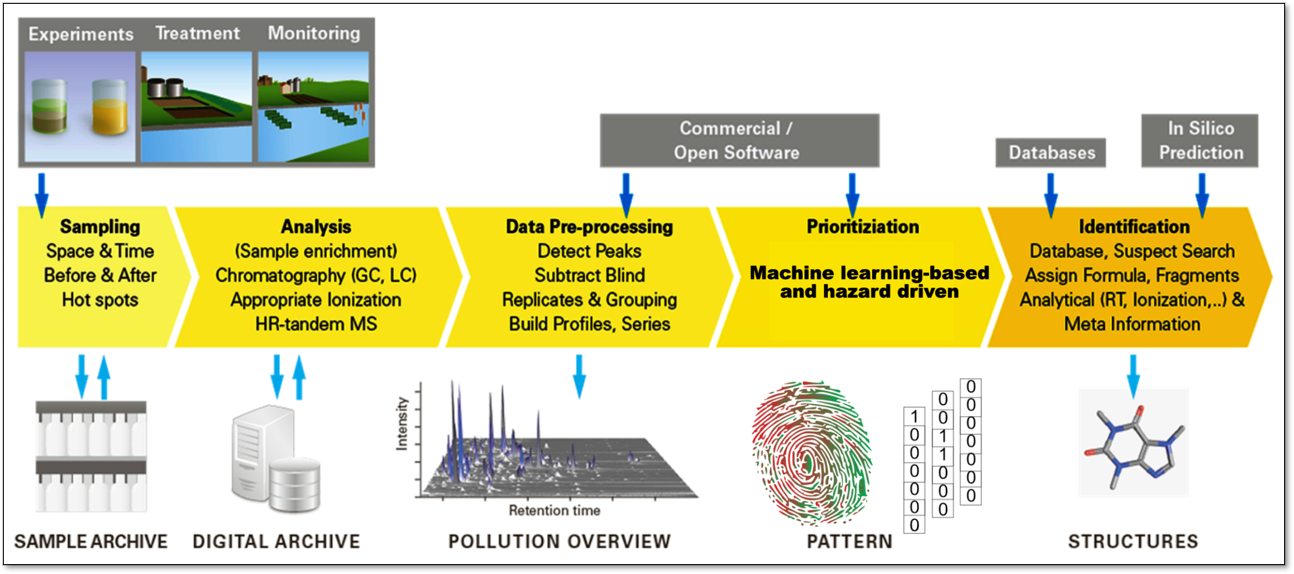
\includegraphics[width=1.0\textwidth]{figures/non_target_high_resolution_mass_spectrometry.png}  
    \caption{Schematic of the workflow used for non-target screening of environmental samples, featuring a customized prioritization step. Adapted from Figure 1 in the original source~\cite{hollender}.}
~\label{fig:non_target_high_resolution_mass_spectrometry} 
\end{figure}

\section{Unlocking the Potential of High-Throughput Screening and Machine Learning in Toxicity Prediction}

In the past few years, the use of machine learning methods has emerged as a transformative force in the field of \emph{in vitro} toxicology, particularly in the realm of high-throughput toxicity prediction.~\emph{High-throughput screening (HTS)} has revolutionized the way toxicity is assessed by allowing thousands of \emph{in vitro} bioassays to be conducted efficiently. This high-throughput approach, coupled with advancements in robotics and automated analysis, has generated large volumes of toxicity data, paving the way for more comprehensive assessments of chemical compounds.
Alongside the rise of machine learning, this advancement has facilitated the creation of predictive models, known as \emph{Quantitative structure-activity relationship (QSAR)} models. These models are capable of forecasting bioactivity or compound toxicity based on their physico-chemical properties or molecular descriptors~\cite{banerjee2018}. As they are trained on extensive datasets containing comprehensive toxicity information, these models can learn the underlying patterns and relationships between chemical structures and target toxicity. With this capability, they can predict the toxicity of new compounds, even when these substances themselves have not undergone laboratory testing. This approach holds the potential to substantially decrease the time and expenses linked to initial toxicity pre-assessment, and it plays a pivotal role in determining which compounds should undergo more in-depth testing.

\begin{figure}[htbp]
    \centering
    \begin{subfigure}[b]{0.48\textwidth}
        \centering
        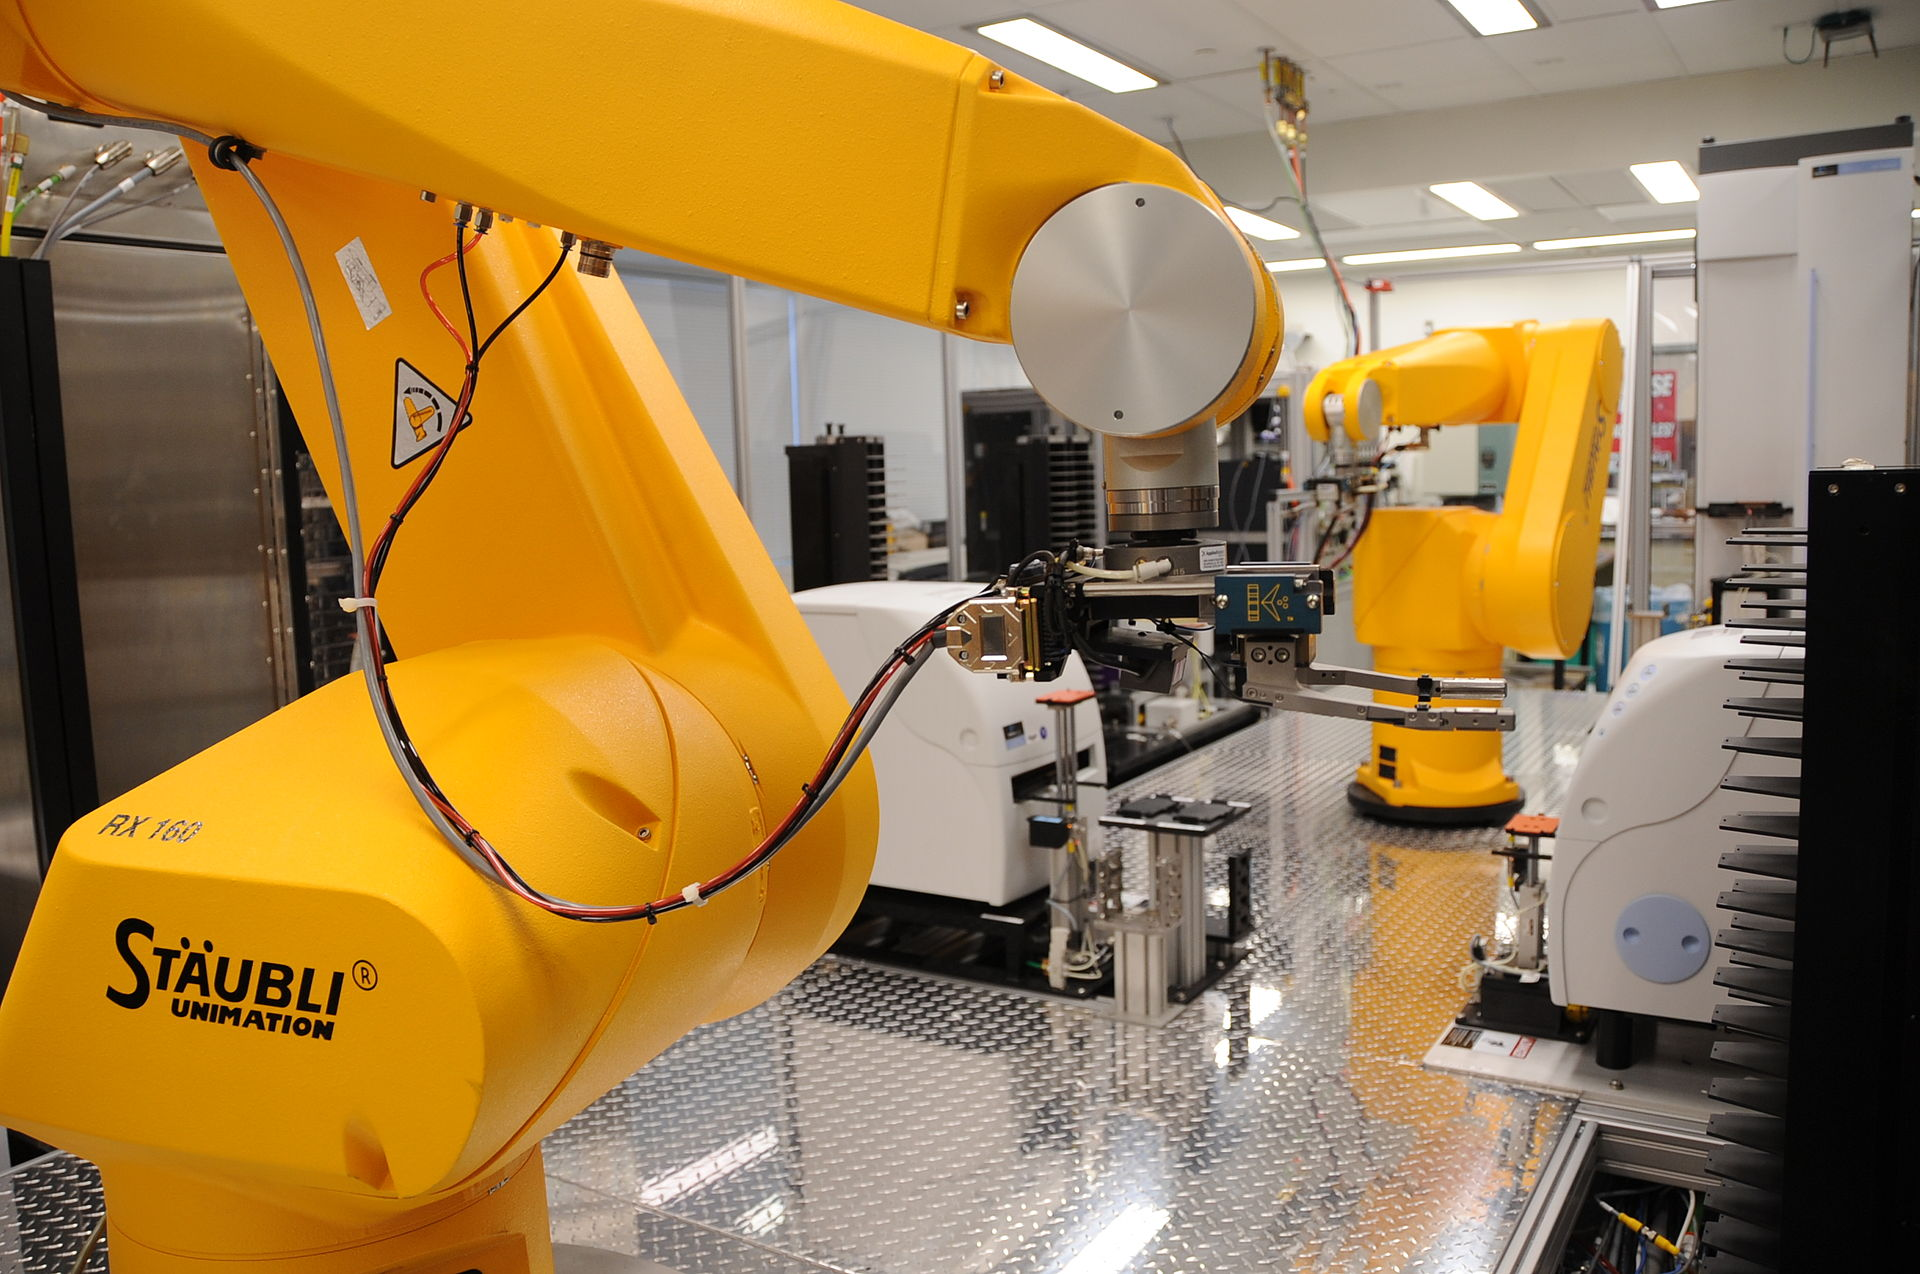
\includegraphics[width=\textwidth]{figures/hts_robot.png}
        \caption{Image obtained from~\cite{hts_robot}. A robot arm retrieves assay plates from incubators and places them at compound transfer stations or hands them off to another arm that services liquid dispensers or plate readers. Efforts in the automation, miniaturization and the readout technologies have enabled the growth of HTS.}
    \label{fig:hts_robot}
    \end{subfigure}
    \hfill
    \begin{subfigure}[b]{0.48\textwidth}
        \centering
        
\includegraphics[width=\textwidth]{figures/hts.png}
        \caption{Image obtained from~\cite{hts_plates}. Modern microtitre assay plates consist of multiples of 96 wells, which are either prepared in the lab or acquired commercially from stock plates. These wells are filled with a dilution solvent, such as \emph{Dimethylsulfoxide (DMSO)}, along with the chemical compounds intended for analysis.}
        \label{fig:hts_plates}
    \end{subfigure}
    \caption{High-Throughput Screening (HTS)}
    \label{fig:hts}
\end{figure}


\section{MLinvitroTox: A Novel Approach}

In response to the pressing need for a more hazard-driven and comprehensive assessment of environmental contaminants, \emph{Arturi et al.} introduced \emph{MLinvitroTox}~\cite{arturi}, an innovative machine learning framework. This framework is part of a broader pipeline named \emph{EXPECTmine}, which incorporates the complementary exposure aspect within the risk assessment process. The primary objective of this thesis is to collaborate with the authors to further enhance and advance this framework. MLinvitroTox leverages molecular fingerprints extracted from fragmentation spectra, marking a significant change in how the toxicity of the myriad unidentified HRMS/MS features is forecasted. MLinvitroTox follows a similar training approach as traditional QSAR models, using supervised classification models trained with molecular fingerprints derived from chemical structures. However, during the application phase, the input to the machine learning model consists of molecular fingerprints generated from experimentally measured\emph{MS2} spectra using \emph{SIRIUS} and \emph{CSI:FingerID}~\cite{sirius2019}. SIRIUS is a software package for annotating small molecules from nontarget HRMS/MS data, while CSI:FingerID is a machine-learning tool employed by SIRIUS to predict molecular fingerprints from fragmentation spectra.Utilizing streamlined machine learning methodologies, MLinvitroTox forecasts chemical toxicity for a wide range of compounds. This comprehensive analysis covers more than 400 target-specific and 70 cytotoxic endpoints, drawing data from ToxCast/Tox21 datasets. Subsequently, the toxicity predictions generated by the framework are employed to prioritize compounds, with the flexibility to emphasize specific aspects of toxicity profiles tailored to individual preferences.

\section{Objectives and Significance}

The main objective of this thesis is to contribute to the development of an efficient MLinvitroTox framework for predicting compound toxicity across multiple endpoints. The goal is to enhance the integration of MLinvitroTox by creating an automated pipeline in the \texttt{Python} programming language. This pipeline is designed to efficiently address the inherent complexities associated with modeling and processing heterogeneous datasets. Here, the emphasis lies in enhancing the curation and filtering of toxicological data and streamlining the process, which begins with raw concentration-response series data and culminates in the generation of the final toxicity predictions. The ultimate output is expected to comprise toxicity fingerprints that encapsulate the predicted toxicity from HRMS/MS environmental samples for the relevant endpoints of interest. These generated toxicity fingerprints will offer crucial insights for the prioritization process, aiding in the identification of the most hazardous compounds present in environmental samples.

One notable contraint of the existing framework lies in its binary \emph{hitcall}  when predicting the toxicity of specific endpoints. It categorizes compounds as either toxic or non-toxic without accounting for variations in toxicity severity. In the long term, it is crucial to adopt a more refined approach that can capture the nuanced continuum of toxicity. This thesis endeavors to overcome this limitation by developing a pipeline capable of forecasting toxicity across numerous endpoints, employing continuous hitcalls.



\section{Thesis Structure}

In the course of progressing through the subsequent chapters, insights will be provided into the materials and methods employed, focusing on the technical intricacies involved in the preparation of ToxCast/Tox21 toxicity data and their transformation into suitable inputs for the machine learning pipeline. This foundational work will establish the basis for the upcoming chapters, which will showcase the potential of MLinvitroTox. Furthermore, the framework's effectiveness is demonstrated through the validation of real-world mass spectral data from \emph{MassBank}~\cite{massbank}, and the examination of the implications of this research is carried out.
